\documentclass[11pt]{article}
\usepackage[margin=1in]{geometry}
\usepackage[T1]{fontenc}
\usepackage{lmodern,microtype,amsmath,amssymb,amsthm,mathtools,booktabs,graphicx,xcolor}
\usepackage{enumitem,fancyhdr,listings,xurl}
\setlength{\emergencystretch}{2em}
\usepackage[numbers,sort&compress]{natbib}
\usepackage[colorlinks=true,linkcolor=teal,citecolor=teal,urlcolor=teal]{hyperref}
\definecolor{teal}{HTML}{087F77}
\definecolor{navy}{HTML}{183D5B}
\hypersetup{pdftitle={Frobenius Lens: Exact Experiment Audits for Periodic Cellular Automata},pdfauthor={Shivam Gupta}}
\newtheorem{theorem}{Theorem}
\newtheorem{proposition}[theorem]{Proposition}
\newtheorem{corollary}[theorem]{Corollary}
\newtheorem{definition}[theorem]{Definition}
\newcommand{\Fp}{\mathbb F_p}
\newcommand{\Obs}{\mathcal O}
\newcommand{\lcmop}{\operatorname{lcm}}
\newcommand{\rank}{\operatorname{rank}}
\newcommand{\ceil}[1]{\left\lceil #1\right\rceil}
\pagestyle{fancy}\fancyhf{}\fancyhead[L]{\small\textsc{Frobenius Lens}}\fancyhead[R]{\small Shivam Gupta}\fancyfoot[C]{\thepage}
\setlength{\headheight}{14pt}
\setlength{\parskip}{4pt}
\setlength{\parindent}{0pt}
\setlist{nosep,leftmargin=*}
\lstset{basicstyle=\ttfamily\small,breaklines=true,frame=single,rulecolor=\color{black!15},columns=fullflexible}
\title{\textbf{Frobenius Lens: Exact Experiment Audits\\for Periodic Cellular Automata}}
\author{Shivam Gupta\\Independent Researcher\\\href{mailto:shivam1720406@gmail.com}{shivam1720406@gmail.com}}
\date{17 October 2026}
\begin{document}
\maketitle
\begin{abstract}
A periodic simulation can agree with a reference on every chosen snapshot while implementing a different local rule. For scalar linear cellular automata over a prime field, we give an exact audit of this ambiguity when snapshots are taken at Frobenius times $t=p^a$. Each experiment---ring length, initial state, and observation time---induces a polynomial divisibility constraint on an undetected rule difference. The least common multiple of these constraints describes the complete ambiguity space of a suite. Its degree determines the observation rank, the number of compatible rules, and a constructive basis of invisible changes. For an impulse on a ring of length $n$, the effective constraint is $x^{n/p^{\min(a,v_p(n))}}-1$: increasing the ring size can add less information than a much smaller change in geometry. A reproducible binary radius-four case leaves 128 rules compatible with snapshots on rings of 32, 64, and 128 cells at time 64. Adding a nine-cell impulse experiment distinguishes all 512 rules; adding a 256-cell ring still leaves 32 compatible. Symbolic certificates agree with direct finite-field calculations across 26,180 exhaustive small configurations and 600 mixed suites; 435 exhaustive fiber checks confirm the predicted ambiguity sizes. A separate browser implementation passes 17,890 checks and supports interactive witnesses and experiment repair. The contribution is a certificate-producing experimental workflow built on classical cellular-automaton algebra, with guarantees restricted to an explicitly declared rule and observation class.
\end{abstract}
\vspace{3pt}
\noindent\textbf{Keywords:} experimental mathematics; cellular automata; finite fields; identifiability; periodic simulation; reproducible software.\\
\textbf{Artifacts:} \url{https://github.com/shi1720/frobenius-lens}

\section{Introduction}
A convincing picture is a useful starting point for mathematical exploration. It is also a measurement produced by a particular initial condition, finite domain, and sampling schedule. Before interpreting agreement between a prototype and a mathematical model, one should ask what those measurements could distinguish even in principle.

Consider a binary linear cellular automaton with nine possible stencil coefficients, at shifts $-4,\ldots,4$. An experiment records the full state after 64 updates from a single impulse on each of three periodic rings, of lengths 32, 64, and 128. These are 224 recorded binary cells. Nevertheless, the measurements impose only two independent constraints on the nine coefficients. Every possible output of this experiment has 128 compatible rules. Increasing the last ring to a larger dyadic geometry helps slowly: adding a 256-cell ring leaves 32 compatible rules. Adding an impulse experiment on nine cells instead determines the rule uniquely.

This is not a floating-point error or an unusual random seed. It follows from the interaction of periodic geometry and the characteristic of the field. A laboratory can repeat the same structurally uninformative experiment indefinitely without resolving the ambiguity. An exploration interface should therefore make the ambiguity visible and suggest an experiment that removes it.

We develop \emph{Frobenius Lens}, a workflow and interactive application for this task. The scope is deliberate: one-dimensional, translation-invariant, scalar linear rules over $\Fp$, known initial states, full-ring observations, and observation times $p^a$, including one. Within this scope the audit is exact and independent of the reference rule. It can be computed before running an experiment.

The contributions are:
\begin{enumerate}
\item A joint experiment certificate, expressed as a least common multiple of seed-dependent polynomial constraints, that characterizes every invisible rule difference and every nonempty observation fiber.
\item A constructive repair formulation and exact small-menu search, together with a sharply resolved example in which a nine-cell experiment supplies information missing from much larger rings.
\item A symbolic prime-field implementation, a separate binary browser implementation, an observation consistency and recovery routine, and a standalone simulator used for independent verification.
\item An exhaustive computational study of the certificate on small spaces, mixed-suite checks, an analytic geometry atlas, and an interactive witness demonstration.
\end{enumerate}
The polynomial representation, Frobenius identity, cyclic-ideal algebra, and linear dependence algorithms used here are established mathematics. The contribution is their combination into an explicit audit-and-repair contract for periodic exploration, rather than a claim to discover those underlying mechanisms.

\section{Related work and the contribution boundary}
\paragraph{Algebraic cellular automata.}
Martin, Odlyzko, and Wolfram represent additive periodic automata through Laurent polynomials modulo $x^n-1$ and analyze periods, predecessors, and transient structure~\cite{martin1984}. Their treatment already contains the finite-field and repeated-factor mechanisms responsible for the examples here. Dennunzio et al. study decidability and dynamical properties of substantially broader additive and matrix-valued classes~\cite{dennunzio2020}. We use the classical scalar setting to ask a different operational question: which \emph{unknown local rules} are observationally equivalent under a specified collection of experiments?

\paragraph{Rule identification.}
Zhao and Billings survey identification from spatiotemporal patterns~\cite{zhao2006}. Sun, Rosin, and Martin estimate local rules and select neighborhoods~\cite{sun2011}; Hafiz et al. formulate identification for cellular automata on spaces of Bernoulli probability measures~\cite{hafiz2025}. These works establish identification as a mature problem. Our object is an exact design-side ambiguity description for a restricted linear class, before parameter estimation or neighborhood learning. We assume that the radius bound and coordinate convention are supplied.

\paragraph{Repeated-root algebra.}
Cyclic codes are described by polynomial ideals, and repeated roots require multiplicity information. Castagnoli et al. develop repeated-root cyclic-code theory and use Hasse derivatives to retain such information~\cite{castagnoli1991}. The same warning matters here: replacing a polynomial by its square-free part can discard experiment constraints. Our factor-exponent ceiling is a direct divisibility calculation, not a new factorization or coding-theory algorithm.

\paragraph{Program search and mathematical applications.}
FunSearch and AlphaEvolve combine program generation with computational evaluators~\cite{funsearch,alphaevolve}. Recent work also examines evaluation-harness design and exploitation~\cite{harness2026}. Our setting isolates one evaluator limitation that exists even with perfectly correct executions: a finite observation map can have a nontrivial kernel. We do not evaluate language-model productivity or the frequency with which coding assistants produce these errors.

Golly, SageMath, and Wolfram Language provide established environments for cellular-automaton exploration~\cite{golly,sage,wolfram}. Frobenius Lens is a small companion diagnostic: its output is a rule-ambiguity certificate and a repair suggestion. We make no comparative usability or feature-completeness claim about those systems. Table~\ref{tab:position} separates the mathematical objects being studied.

\begin{table}[t]
\centering\small
\caption{Position of the present work. The table compares questions, not performance.}
\label{tab:position}
\begin{tabular}{@{}p{.27\linewidth}p{.30\linewidth}p{.35\linewidth}@{}}
\toprule
Line of work & Principal object & Object audited here\\\midrule
Classical CA algebra~\cite{martin1984} & Dynamics of a known rule & Ambiguity among bounded unknown rules\\
Rule identification~\cite{sun2011,zhao2006} & Rule/neighborhood estimation & Exact equivalence under a declared design\\
Repeated-root codes~\cite{castagnoli1991} & Code ideals and distance & Frobenius preimages of seed annihilators\\
Program search~\cite{funsearch,alphaevolve} & Programs evaluated by a harness & Information retained by a snapshot harness\\
Exploration environments~\cite{golly,sage,wolfram} & Simulation and visualization & Invisible changes and additional experiments\\\bottomrule
\end{tabular}
\end{table}

\section{Rules, experiments, and observations}
Let $p$ be prime and $r\geq0$ a declared radius bound. The rule class is
\begin{equation}
\mathcal F_r=\left\{f(x)=\sum_{j=-r}^{r}c_jx^j:c_j\in\Fp\right\}.
\end{equation}
The bound is inclusive: endpoint coefficients may vanish. Thus $|\mathcal F_r|=p^{2r+1}$. Multiplication by $f$ means the local update
\begin{equation}
 u_i^{(k+1)}=\sum_{j=-r}^{r}c_j u_{i-j}^{(k)}\pmod p,
 \qquad i\in\mathbb Z/n\mathbb Z.
 \label{eq:update}
\end{equation}
The sign of the shift is fixed by this equation. We do not identify rules up to reflection, spatial shift, or a change of origin.

An experiment $e=(n,t,s)$ consists of a positive ring length $n$, a time $t=p^a$ with $a\geq0$, and a known initial-state polynomial $s\in\Fp[x]$ of degree less than $n$. The zero seed is permitted. Write $M_n=x^n-1$ and $R_n=\Fp[x]/(M_n)$. Since $x$ is a unit in $R_n$, Laurent rules act on this quotient without ambiguity. The full observation is
\begin{equation}
 \Obs_e(f)=f(x)^t s(x)\pmod{M_n}.
 \label{eq:obs}
\end{equation}
For a finite suite $E$, $\Obs_E$ concatenates the full observations from its experiments. Each experiment starts afresh from its specified seed; snapshots are indexed by absolute time from that seed. The observations are exact field elements, rather than rendered pixels, histograms, or noisy measurements.

Define the normalized rule $F=x^rf\in\Fp[x]$, with $\deg F\leq d:=2r$. For two rules $f,g$, write $H=x^r(f-g)$. At a Frobenius time,
\begin{equation}
 f^t-g^t=(f-g)^t=x^{-rt}H^t.
 \label{eq:frobenius}
\end{equation}
Consequently, $\Obs_E$ is linear over $\Fp$ in the $d+1$ rule coefficients. This is linearity in the \emph{rule}, in addition to the usual linearity in the state. Equation~\eqref{eq:frobenius} is the reason for restricting the time domain. It generally fails at other times.

\section{An exact certificate for the whole suite}
For each experiment define
\begin{equation}
 q_e=\frac{M_n}{\gcd(M_n,s)}=\prod_{\phi}\phi^{v_{e,\phi}},
 \qquad
 Q_e=\prod_{\phi}\phi^{\ceil{v_{e,\phi}/t}},
 \label{eq:Q}
\end{equation}
where the factors are monic irreducible polynomials over $\Fp$. Empty products are one. Define the joint polynomial
\begin{equation}
 L_E=\lcmop_{e\in E}Q_e,\qquad D_E=\deg L_E,
 \label{eq:L}
\end{equation}
with $L_\varnothing=1$. This certificate depends only on the design, not on the unknown rule or its measured output.

\begin{theorem}[Complete ambiguity certificate]\label{thm:main}
For every suite $E$ in the stated scope and every $f,g\in\mathcal F_r$,
\begin{equation}
 \Obs_E(f)=\Obs_E(g)
 \quad\Longleftrightarrow\quad L_E\mid x^r(f-g).
 \label{eq:equiv}
\end{equation}
The coefficient-space kernel has dimension
\begin{equation}
 \nu_E=\max\{0,d+1-D_E\},
 \qquad \rank\Obs_E=d+1-\nu_E.
 \label{eq:rank}
\end{equation}
Every nonempty observation fiber contains exactly $p^{\nu_E}$ rules. The suite distinguishes every rule in $\mathcal F_r$ if and only if $D_E>d$. When $\nu_E>0$, a basis of normalized invisible differences is
\begin{equation}
 L_E,xL_E,\ldots,x^{d-D_E}L_E.
 \label{eq:basis}
\end{equation}
\end{theorem}
\begin{proof}
Fix an experiment and put $M=M_n$. Equations~\eqref{eq:obs}--\eqref{eq:frobenius} show that equality of observations is equivalent to $M\mid H^t s$, since $x^{-rt}$ is a unit modulo $M$.

Let $z=\gcd(M,s)$, $M=zq$, and $s=zs'$. Then $\gcd(q,s')=1$, so $M\mid H^t s$ is equivalent to $q\mid H^t$. For every irreducible $\phi$, this is equivalent to $t\,v_\phi(H)\geq v_\phi(q)$, or $v_\phi(H)\geq\ceil{v_\phi(q)/t}$. Hence the equality holds exactly when $Q_e\mid H$. Requiring this for all experiments gives $L_E\mid H$.

If $D_E>d$, no nonzero polynomial of degree at most $d$ is divisible by $L_E$. Otherwise the admissible multiples are exactly $L_E B$, with $\deg B\leq d-D_E$. Multiplication by the nonzero polynomial $L_E$ is injective in $\Fp[x]$, and the monomials in $B$ give the basis~\eqref{eq:basis}. This establishes the kernel dimension and, by rank--nullity, the rank. A nonempty fiber of a linear map is a coset of its kernel, so its size is $p^{\nu_E}$.
\end{proof}

Theorem~\ref{thm:main} characterizes a finite model class exactly. It does not infer that a black-box program implements a member of that class. If observations are inconsistent with the class, there is no compatible rule and the fiber-size statement does not apply. The software checks consistency separately when recovering coefficients.

\begin{figure}[t]
\centering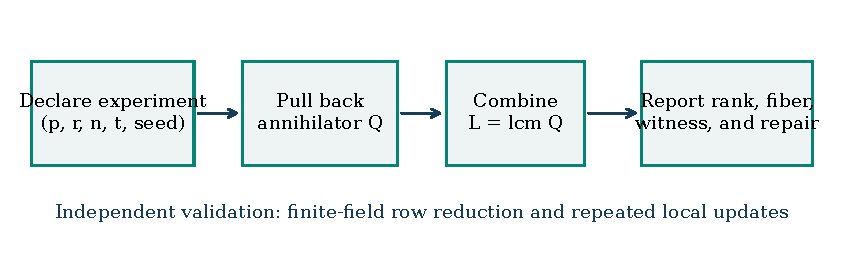
\includegraphics[width=\linewidth]{../figures/pipeline.pdf}
\caption{The audit contract. A design determines $Q_e$ and $L_E$ before any unknown-rule observations are used. Independent numerical paths verify the bounded computational study.}
\label{fig:pipeline}
\end{figure}

\subsection{Impulse probes and the effective ring length}
\begin{corollary}[Exact impulse reduction]\label{cor:impulse}
For an impulse $s=1$, let $n=p^b m$ with $p\nmid m$ and $t=p^a$. Then
\begin{equation}
 Q_e=(x^m-1)^{p^{\max(b-a,0)}}
     =x^{n/p^{\min(a,b)}}-1.
 \label{eq:effective}
\end{equation}
An impulse suite therefore uses the least common multiple of the polynomials in~\eqref{eq:effective}. A single impulse experiment is identifying exactly when $n/p^{\min(a,b)}>2r$.
\end{corollary}
\begin{proof}
In characteristic $p$, $x^n-1=(x^m-1)^{p^b}$. Since $p\nmid m$, the polynomial $x^m-1$ is square-free: its derivative $mx^{m-1}$ is relatively prime to it. Every irreducible multiplicity is $p^b$. Equation~\eqref{eq:Q} replaces it by $\ceil{p^b/p^a}=p^{\max(b-a,0)}$. Applying Frobenius again gives the final expression. Theorem~\ref{thm:main} supplies the threshold.
\end{proof}

For $p=2$, a ring of $2^b$ cells observed at $2^a$ with $a\geq b$ supplies only the constraint $x-1$. In contrast, an odd ring retains $Q_e=x^n-1$ at every supported time. The geometry atlas in Figure~\ref{fig:landscape} shows this arithmetic structure. Neighboring ring sizes can have very different information content even when they look equally adequate as display resolutions.

\begin{figure}[t]
\centering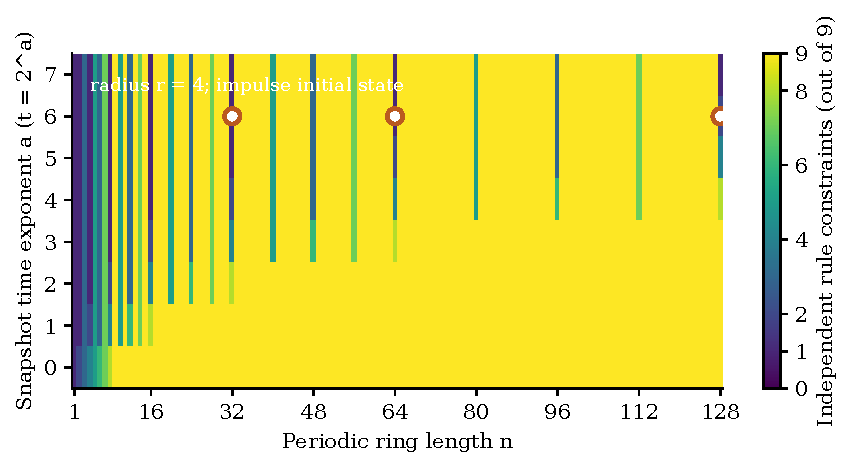
\includegraphics[width=\linewidth]{../figures/landscape.pdf}
\caption{Exact analytic rank for a binary radius-four rule under one impulse experiment. The color is $\min(9,n/2^{\min(a,v_2(n))})$. Circled cells mark the three time-64 experiments in the case study. The image shows a formula, not a sampled error rate.}
\label{fig:landscape}
\end{figure}

\subsection{What additional seeds and later snapshots can change}
\begin{proposition}[Limits of repetition]\label{prop:repeat}
On a fixed ring, the union of any seed experiments at a fixed Frobenius time cannot impose a stronger constraint than an impulse at that time. For a fixed seed and ring, adding later Frobenius times to an earlier Frobenius snapshot adds no rule information. An all-one initial state gives $Q_e=x-1$ at every supported time; a zero state gives $Q_e=1$.
\end{proposition}
\begin{proof}
For every seed, $q_e\mid M_n$, so the factor-exponent ceilings in its $Q_e$ do not exceed those of the impulse constraint. Their least common multiple also divides that constraint. At a later Frobenius time, each ceiling is no larger than at the earlier time, so the later constraint divides the earlier one. Finally, the all-one seed is $s=(x^n-1)/(x-1)$, giving $q_e=x-1$, whose ceiling remains one. A zero seed has $q_e=1$.
\end{proof}

This does not say that extra seeds are useless when the original seed is weak. An impulse can recover information omitted by a constant state. It says that once an impulse has supplied the entire operator response at a fixed time, more initial states cannot recover a rule difference whose time-$t$ operator is already zero. Figure~\ref{fig:seeds} distinguishes these two sources of lost information.

\begin{figure}[t]
\centering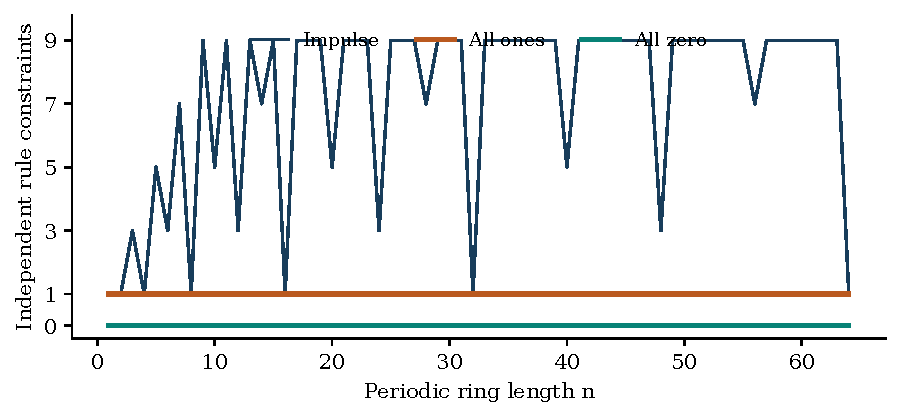
\includegraphics[width=\linewidth]{../figures/seed_effect.pdf}
\caption{Seed effects for binary radius four at time 64. Full-ring observations of all-one states constrain only the coefficient sum, even on odd rings. All-zero states impose no constraint. Impulse probes expose the geometry-dependent maximum for a fixed ring and time.}
\label{fig:seeds}
\end{figure}

\begin{proposition}[Detection by a random seed]\label{prop:random}
Fix distinct rules with normalized difference $H$, and a ring/time pair $(n,t)$ in scope. If the initial state is uniform on $\Fp^n$, the probability of equal observations is
\begin{equation}
 \Pr\{\Obs_e(f)=\Obs_e(g)\}
 =p^{-\left(n-\deg\gcd(M_n,H^t)\right)}.
 \label{eq:random}
\end{equation}
For $k$ independently chosen initial states on the same ring and time, the exponent is multiplied by $k$. If $M_n\mid H^t$, the probability remains one for every $k$.
\end{proposition}
\begin{proof}
Put $G=\gcd(M_n,H^t)$. The condition $M_n\mid H^t s$ is equivalent to $(M_n/G)\mid s$. Exactly $p^{\deg G}$ polynomials of degree less than $n$ satisfy this condition. Divide by $p^n$ and use independence for repetitions.
\end{proof}
This is a probability conditional on an explicitly uniform seed model. It is not an estimated prevalence of errors in real mathematical software.

\section{Repairing an experiment design}
Let $\mathcal C$ be a finite menu of additional experiments with positive costs $w_e$. Given an existing suite $E$, a complete repair solves
\begin{equation}
 \min_{S\subseteq\mathcal C}\sum_{e\in S}w_e
 \quad\text{subject to}\quad
 \deg\lcmop\bigl(L_E,\{Q_e:e\in S\}\bigr)>d.
 \label{eq:repair}
\end{equation}
The cost can represent stored cells, simulation work, or an externally supplied resource measure. These are different objectives. The case study uses $w_e=n_e$, the number of newly stored snapshot cells. It does not equate this quantity with runtime.

A simple necessary lower bound is
\begin{equation}
 \sum_{e\in S}n_e\geq\max(0,d+1-D_E),
 \label{eq:lower}
\end{equation}
because $\deg\lcmop(L_E,\{Q_e\})\leq D_E+\sum_e\deg Q_e\leq D_E+\sum_e n_e$. Overlap between factors can make the bound strict. In particular, summing individual experiment degrees without subtracting common factors is not a valid certificate.

The reference implementation enumerates subsets and retains the cheapest feasible repair; it caps the menu at 22 entries. This is an exponential exact search for small menus. We do not claim a polynomial-time global design algorithm. The browser demonstration instead scans increasing ring lengths for the cheapest \emph{single impulse} addition in a finite range. A result from that scan is not labeled optimal over all seeds, times, or multisets of experiments.

\subsection{A fully resolved radius-four example}
Set $p=2$, $r=4$, and take impulse experiments on rings 32, 64, and 128, all at time 64. Their constraints are $x+1$, $x+1$, and $(x+1)^2$, so $L_E=x^2+1$, $D_E=2$, and $\nu_E=7$. A concrete invisible normalized difference is $H=x^2+1$. For example,
\begin{align}
 F&=1+x^2+x^3+x^6+x^8,\\
 G&=F+H=x^3+x^6+x^8.
\end{align}
The corresponding physical rules are $f=x^{-4}F$ and $g=x^{-4}G$. Their histories can differ at intermediate times while their declared snapshots agree (Figure~\ref{fig:witness}).

For an additional nine-cell impulse experiment at time 64, $Q=x^9+1$ and
\begin{equation}
 \lcmop(x^2+1,x^9+1)=(x+1)(x^9+1)
 =x^{10}+x^9+x+1.
\end{equation}
Its degree ten exceeds eight; therefore all 512 rules are distinguished. The fixed witness differs in two of the nine final cells.

Among additional single impulse rings at this same time, nine is the smallest successful length. For $n\leq8$, the effective lengths are $1,1,3,1,5,3,7,1$. Combining each resulting constraint with $x^2+1$ gives degree at most eight. Length nine gives degree ten. If every new ring must have at most seven cells, rings three and seven together achieve degree ten and cost ten. Exhaustive subset search of the seven-entry menu proves that no lower-cost subset in that menu is sufficient. These are concrete optimality statements under declared menus and costs.

\begin{figure}[t]
\centering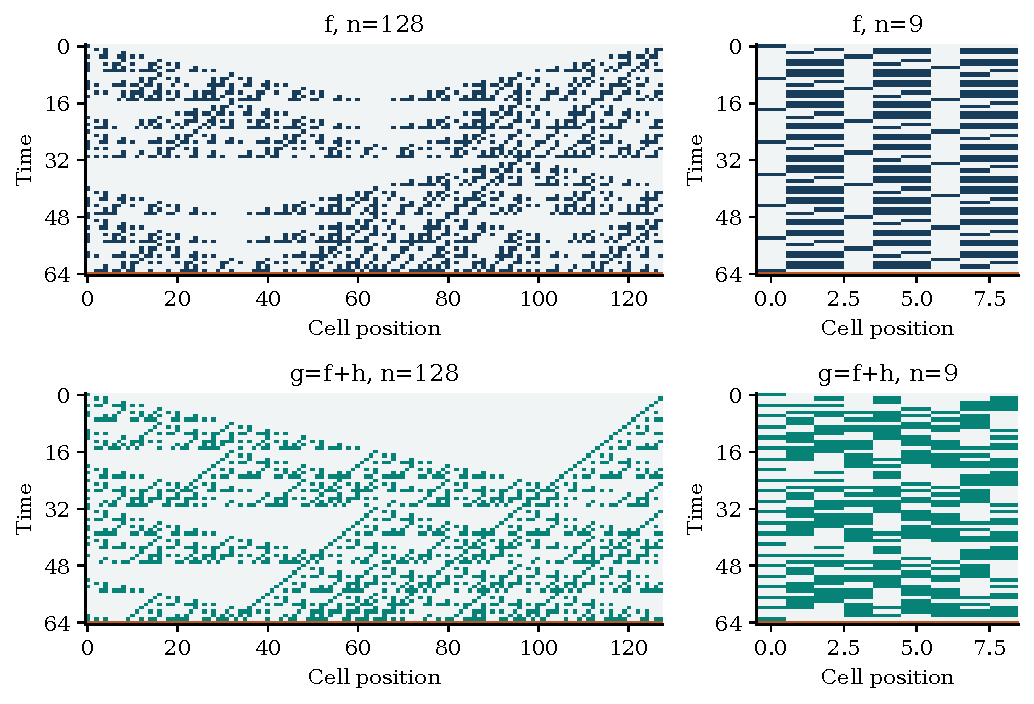
\includegraphics[width=\linewidth]{../figures/witness.pdf}
\caption{Direct simulation of the two displayed rules from an impulse. The horizontal line marks time 64. On the 128-cell ring, both final states coincide despite different histories. On nine cells, their final states differ. These images visualize an exact witness established algebraically and checked by repeated local updates.}
\label{fig:witness}
\end{figure}

\begin{figure}[t]
\centering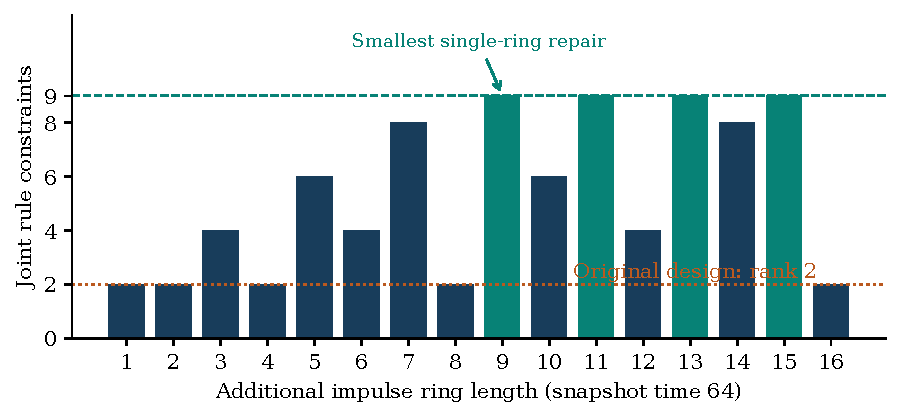
\includegraphics[width=\linewidth]{../figures/repair.pdf}
\caption{Joint rank after adding one impulse experiment at time 64 to the original three-ring suite. Nine is the smallest additional ring attaining rank nine. More recorded cells do not imply a more informative geometry: powers of two remain weak at this time.}
\label{fig:repair}
\end{figure}

\section{Implementation and independent verification}
The Python implementation uses exact polynomial gcd, factorization, and least common multiple operations in SymPy 1.14.0. For each experiment it constructs $q_e$, replaces every irreducible multiplicity $v$ by $\ceil{v/t}$, and accumulates $L_E$. It exports field coefficients in increasing degree order, experiment specifications, the joint generator, rank, nullity, fiber size, and a kernel basis. The core certificate procedure is:
\begin{lstlisting}[caption={Certificate construction; all polynomial operations are over the declared prime field.}]
L = 1
for (n, t, seed) in experiments:
    require t is a power of p
    M = x**n - 1
    q = exact_quotient(M, gcd(M, seed))
    Q = product(phi**ceil(v/t) for phi, v in factor(q))
    L = monic(lcm(L, Q))
nullity = max(0, 2*radius + 1 - degree(L))
return L, nullity, [x**j * L for j in range(nullity)]
\end{lstlisting}

A separate \texttt{recover} routine forms the linear observation equations, rejects inconsistent full-ring observations, and returns one compatible coefficient vector plus the ambiguity certificate. Recovery uses modular Gaussian elimination. It does not force a unique answer when the design is underdetermined.

The browser implementation is restricted to $p=2$ and uses BigInt polynomial arithmetic. It obtains $Q_e$ without factorization: starting with $s,x^t s,x^{2t}s,\ldots$ modulo $M_n$, it finds the first vector dependence, tracking the dependence coefficients. This is a standard Krylov dependence construction. At binary Frobenius times the dependence polynomial is precisely the smallest-degree monic $H$ with $H^t s=0$, hence $Q_e$. Section~\ref{app:krylov} gives the argument. Euclidean polynomial operations then produce the joint least common multiple.

The independent Python verifier imports neither SymPy nor the certificate module. It implements Equation~\eqref{eq:update} with lists, constructs observation-matrix columns by evolving each coefficient-basis rule, and calculates rank by modular row reduction. Exhaustive fiber checks instead enumerate every rule and group identical simulated outputs. These paths have different failure modes: symbolic factor arithmetic, local stepping, linear elimination, and output partitioning.

The artifact includes a protocol file, raw per-configuration results, deterministic random seeds, code, figure-generation scripts, and test summaries. It is designed for replay rather than reliance on screenshots or aggregate numbers alone.

\section{Computational results}
All reported experiments were executed with Python 3.12.14 on an arm64 macOS machine. The primary run took 69.14 seconds. This duration describes one local run and is not a portable speed guarantee. The protocol hash and raw results are in the repository.

\subsection{Exhaustive small-space audit}
The primary grid covers every binary seed for ring lengths $1\leq n\leq9$, times $1,2,4,8$, and radii $0,1,2,3$: 16,352 configurations. A second grid covers every ternary seed for $1\leq n\leq6$, times $1,3,9$, and radii $0,1,2$: 9,828 configurations. Zero seeds and rings shorter than the stencil are included. Predicted rank agrees exactly with independently simulated rank in all 26,180 configurations.

For mixed designs, 400 binary and 200 ternary suites use a deterministic pseudorandom generator seeded with 1720406. Each contains one to four experiments; radii range from zero through eight, ring lengths from one through 24, and time exponents from zero through three. There are no rank disagreements. Random here describes the constructed design generator, not an assumption used in Theorem~\ref{thm:main}.

An additional 435 configurations enumerate the entire rule class and compare actual fiber sizes to $p^{\nu_E}$. Binary radii one through three use rings one through six, four supported times, and five seed choices. Ternary radius one uses rings one through five, three times, and five seed choices. The choices are zero, impulse, constant, alternating, and fixed pseudorandom; duplicate seeds are retained and counted as repeated test configurations. Every partition has the predicted number and uniform size of nonempty fibers.

\begin{table}[t]
\centering\small
\caption{Executed exact checks. Counts refer to assertions or design configurations as specified, not independent statistical samples.}
\label{tab:checks}
\begin{tabular}{@{}p{.62\linewidth}rr@{}}
\toprule
Check & Count & Failures\\\midrule
Exhaustive single-experiment rank configurations & 26,180 & 0\\
Mixed-suite rank configurations & 600 & 0\\
Polynomial snapshot vs. repeated local updates & 1,545 & 0\\
Constructive kernel witnesses & 975 & 0\\
Exhaustive observation-fiber configurations & 435 & 0\\
Impulse formula grid ($p=2,3,5$) & 2,304 & 0\\
Case-study fibers and repair searches & 7 & 0\\
Input guards and non-Frobenius counterexample & 5 & 0\\\midrule
Primary Python assertions & 32,051 & 0\\
Separate browser-kernel checks & 17,890 & 0\\\bottomrule
\end{tabular}
\end{table}

The 2,304-point impulse grid compares the symbolic certificate with Equation~\eqref{eq:effective} for $p\in\{2,3,5\}$, $1\leq n\leq128$, and $0\leq a\leq5$. It is a cross-check of two algebraic formulations, whereas the exhaustive small grids use independent local simulation. Table~\ref{tab:checks} preserves that distinction. Ten additional unit-test methods cover boundaries, duplicates, empty suites, inconsistent data, unsupported domains, and recovery. The recovery method tests 180 field/radius/ring/time combinations.

The browser kernel agrees with all 16,352 binary rank/degree fixtures. It also agrees with repeated JavaScript time stepping on 1,536 rule/geometry/time combinations and passes two case-study fiber checks, for 17,890 checks in total. UI inspection confirms that applying the suggested nine-cell repair changes the displayed rank from two to nine and the fiber size from 128 to one.

\subsection{Exhaustive repair comparison}
Table~\ref{tab:repair} enumerates every one of the 512 radius-four binary rules for each design, relative to the fixed target in Section~5.1. An alternative is missed exactly when its entire recorded output equals that of the target. These are exhaustive counts over the declared class; they are not measurements of naturally occurring implementation errors.

\begin{table}[t]
\centering\small
\caption{Exact design comparison. Added cells count newly stored full snapshots, beyond the original 224 cells. Each row starts from the same original suite.}
\label{tab:repair}
\begin{tabular}{@{}p{.37\linewidth}rrrr@{}}
\toprule
Additional experiment(s) & Added cells & Rank & Fiber & Missed alternatives\\\midrule
None & 0 & 2 & 128 & 127\\
$n=256$, $t=64$, impulse & 256 & 4 & 32 & 31\\
$n=128$, $t=1$, impulse & 128 & 9 & 1 & 0\\
$n=9$, $t=64$, impulse & 9 & 9 & 1 & 0\\
$n=3,7$, $t=64$, impulses & 10 & 9 & 1 & 0\\\bottomrule
\end{tabular}
\end{table}
The earlier snapshot is a valid and effective control. The repair's advantage in this example is that it preserves the late observation time while using fewer additional snapshot cells. Recording the first update is often the simpler choice when the interface permits it. The result does not justify preferring late sampling in general.

\subsection{Descriptive computation cost}
For binary radius four at time 64, five local repeats gave median cached-certificate times of 0.92, 1.02, 0.92, and 0.87 milliseconds for ring lengths 32, 64, 128, and 256. Independent basis simulation and rank computation took 4.90, 10.64, 19.32, and 30.54 milliseconds. The certificate timings reuse the cached per-experiment factorization; the basis simulation timings perform time stepping. They are different tasks, not an end-to-end algorithmic speed comparison. The raw repeats are provided to make this qualification inspectable. The mathematical information result does not depend on these timings.

\section{Interactive use and practical applications}
A workshop demonstration begins with the three-ring design and asks whether 224 recorded cells determine nine coefficients. The app reports two independent constraints, an ambiguity dimension of seven, and 128 compatible rules. It displays $L_E=x^2+1$ and a concrete pair of distinct rules with identical recorded snapshots. A user can inspect their histories, request a repair, and apply the nine-cell experiment. The witness is retained after the repair, making the newly detected difference visible.

Changing the initial state to all ones exposes a different issue: a geometrically adequate ring can still provide only one constraint. Changing the radius shows the boundary between a complete and an incomplete design. Exported JSON records the experiment assumptions, coefficients of $L_E$, rank, nullity, and fiber size. The local browser app requires neither a server-side model nor a network connection after loading its two static files.

There are three concrete integration opportunities. First, a mathematical notebook can attach the certificate to a conjecture-generating simulation so that the domain and sampling assumptions remain visible. Second, a regression harness for finite-field stencil software can choose a complete impulse design rather than accumulate redundant late snapshots. Third, an educational environment can turn an apparently anomalous simulation into a constructive lesson about characteristic, repeated roots, and identifiability.

A commercial implementation could package these checks as a notebook extension or testing component for computational-science tooling. The present artifact establishes an exact restricted capability and a reproducible demonstration. It does not establish customer demand, willingness to pay, a market-size estimate, or superiority over existing commercial tools. The adjacent product landscape contains mature simulators and symbolic environments~\cite{golly,sage,wolfram}; a credible product hypothesis is integration with these workflows. A next validation step would be a corpus of real simulation revisions with separately verified rule-class membership and resource accounting.

\section{Limitations and scope of the evidence}
The strongest conclusion is conditional and finite: under the declared scalar linear class and exact full observations, the certificate completely characterizes rule ambiguity. Several boundaries matter in use.

\textbf{Rule-class membership.} A nonlinear implementation, an asynchronous update, a boundary bug, or a state-dependent stencil can agree on the certified experiments without belonging to $\mathcal F_r$. One must establish the intended class separately, for example through source inspection or a restricted implementation language. A complete certificate for $\mathcal F_r$ is not a proof of arbitrary-program correctness.

\textbf{Observation scope.} Cropped views, screenshots, population counts, noisy measurements, unknown initial states, and unknown spatial alignment are outside the theorem. The software consumes full vectors of exact field elements. A rendered figure is an illustration, not the observation oracle.

\textbf{Time and algebra.} The proof uses $t=p^a$. At time three in characteristic two, $(f+g)^3$ generally differs from $f^3+g^3$; the artifact includes a concrete counterexample and rejects that time in the certificate API. Matrix-valued rules introduce noncommuting coefficient operations, and multidimensional polynomial rings do not generally admit a single principal generator. Neither extension follows from the present proof.

\textbf{Novelty and scale.} The algebra is classical. The proposed contribution is an executable, seed-aware, multi-experiment audit with complete ambiguity reporting and repair. The literature review supports this positioning; it cannot prove that every equivalent formulation is absent from the literature. The exhaustive checks are finite and share ordinary software/hardware risks. They corroborate the proofs but do not replace them, nor do they establish widespread practical error rates.

\textbf{Design optimization.} The subset search is exponential and intended for small menus. Snapshot-cell cost omits many real deployment costs. A more expensive experiment in this metric can be preferable when runtime, visualization, or existing infrastructure dominates.

\section{Conclusion}
Periodic experiments should be accompanied by a statement of what they distinguish. For scalar linear cellular automata at Frobenius times, that statement can be exact: a polynomial $L_E$ determines every invisible rule change, the observation rank, and the size of every compatible-rule set. The nine-cell repair demonstrates why a small change in experiment geometry can resolve ambiguity that persists across much larger simulations. Frobenius Lens makes this algebra available as a working exploration tool, with proofs, raw finite checks, and separate implementations that can be inspected and reproduced.

\paragraph{Code and data availability.}
The repository at \url{https://github.com/shi1720/frobenius-lens} contains source, protocol, raw results, tests, browser app, and figure/manuscript sources. Software is released under the MIT license. Generated results are deterministic except for recorded wall-clock timings. No proprietary data are required.

\bibliographystyle{plainnat}
\bibliography{references}
\clearpage
\appendix
\section{Factorization-free binary certificate}\label{app:krylov}
For a binary experiment $(n,t,s)$ with $t=2^a$, let $V_j=x^{jt}s\pmod{x^n-1}$. Perform exact elimination on $V_0,V_1,\ldots$, retaining the binary linear combination used in every elimination. At the first dependence index $k$, write
\begin{equation}
 V_k+\sum_{j=0}^{k-1}b_jV_j=0,
 \qquad B(x)=x^k+\sum_{j=0}^{k-1}b_jx^j.
\end{equation}
Frobenius gives $B(x)^t s=V_k+\sum_j b_jV_j=0$. Therefore $Q_e\mid B$ by the argument of Theorem~\ref{thm:main}. Conversely, $Q_e^t s=0$ supplies a dependence at index $\deg Q_e$. Minimality implies $k=\deg Q_e$, and the two monic polynomials agree. A dependence exists by index $n$, since all vectors lie in an $n$-dimensional space. For a zero seed it occurs at index zero and returns $Q_e=1$.

The browser represents vectors and dependence polynomials as BigInts, uses bitwise xor for addition, and implements binary Euclidean division for gcd and least common multiple. The algorithm is deterministic. Its worst-case work grows with the ring dimension and is not claimed to improve on specialized algebraic algorithms. The UI caps ring length at 512 and the displayed radius at 12; the kernel API accepts radii up to 32.

\section{A non-Frobenius counterexample}
Take $p=2$, $n=7$, and radius one, with normalized coefficient vectors $(1,1,0)$ and $(0,1,1)$. In Laurent notation these are $f=x^{-1}+1$ and $g=1+x$. At time three,
\begin{equation}
 (f+g)^3-f^3-g^3=f^2g+fg^2
  =x^{-2}+x^2\neq0\pmod{x^7-1}.
\end{equation}
An impulse therefore observes a nonlinear-in-rule map. The linear fiber argument must not be extended to this time by simply replacing $t$ in Equation~\eqref{eq:Q}. For example, the factorization $f^t-g^t=(f-g)^t$ used in the main proof is already false.

\clearpage
\section{Reproduction map}
The artifact paths are relative to the repository root.
\begin{table}[h]
\centering\small
\begin{tabular}{@{}p{.44\linewidth}p{.48\linewidth}@{}}
\toprule
Path & Purpose\\\midrule
\texttt{src/frobenius\_lens.py} & Exact prime-field certificate, snapshots, repair, recovery\\
\texttt{tests/independent.py} & Separate local-update simulator and modular rank\\
\texttt{experiments/protocol.json} & Primary finite grids, seed, and case specification\\
\texttt{experiments/run.py} & Execute primary checks and save raw results\\
\texttt{results/single\_checks.csv} & Every exhaustive single-design rank comparison\\
\texttt{results/suite\_checks.json} & Mixed-suite specifications and certificates\\
\texttt{results/fiber\_checks.json} & Exhaustive output-partition results\\
\texttt{results/case\_study.json} & Compatible rule IDs and exact repair outcomes\\
\texttt{app/lens.mjs} & Factorization-free binary browser kernel\\
\texttt{tests/test\_browser\_kernel.mjs} & Browser-kernel fixture and time-stepping checks\\
\texttt{experiments/figures.py} & All five vector figures in the manuscript\\\bottomrule
\end{tabular}
\end{table}

A minimal exact audit is:
\begin{lstlisting}[language=Python]
from frobenius_lens import Experiment, certificate
E = [Experiment(n, 64) for n in (32, 64, 128)]
assert certificate(E, radius=4)["fiber_size"] == 128
E.append(Experiment(9, 64))
assert certificate(E, radius=4)["fiber_size"] == 1
\end{lstlisting}
The primary protocol SHA-256 is
\begin{center}\small\ttfamily
28873bd3abc7d1cf75668cd251f76595b6d\\
1642ff49db10c143cc55ba60495c1.
\end{center}
This identifies the protocol text, not a public preregistration. The UI and recovery checks were added as implementation validation alongside the primary study.

\end{document}
